The arrival and diffusion of Internet has revolutionized the world in which we live in and has introduced, along with many other things, a new way of learning. With time, the first E-Learning services were devoloped and throughout the years they have evolved and are now commonly called MOOC (Massive Open Online Course).

The main difference between MOOC platforms today and in the past is that they generally offer open courses to anyone, in which the participation is free and they allow interactivity among the students.

The enormous potential of these systems has been noticed straight away and already in 2012 these services were about 100 and almost 700 in 2013, with an average of 2 new MOOCs per day.

It has been estimated that the turnover linked with E-Learning in 2012 alone was 35.6 billion dollars.\cite{gallico2015learning}.
Considering, however, the high number of platforms present, the market is very fragmented. Nonetheless, the most important part is taken up by the main platforms such as Coursera, EdX, Udacity, Udemy and SkillShare.

Some of the most prestigious universities, such as Standford, Harvard, Berkeley and MIT, use these platforms to deliver part of their own formative educational plans and extend their catchment area.
The courses offered cover various themes and are delivered directly to the professors of said universities.

The business model of these services consents the free access following the classic MOOC philosophy. A monetary fee is asked only if someone would like to have a certificate, which is released only after having passed an exam that verifies the actual learning level of the person.

MOOC has eliminated temporal and spatial barriers and has the merit of simplifying the access to a university training. They are often invoked as contributors when not directly makers of an actual revolution of the educational world.

During the last years, there has been a diffusion of an alternative model referred to the one introduced up until now: instead of an authoritative entity in the formation field, such as a prestigious university which delivers a course by one of their professors, some platforms are introducing the possibility of structuring an online course for anyone who is interested.

This is, for example, the case of Udemy, which has encountered a great success and has been used by many people who have published numerous courses on the platform. Some of these courses are accessible only after a payment has been made, thus becoming an actual profit for the professor.

\begin{figure}[htb] %  figure placement: here, top, bottom
 \centering
 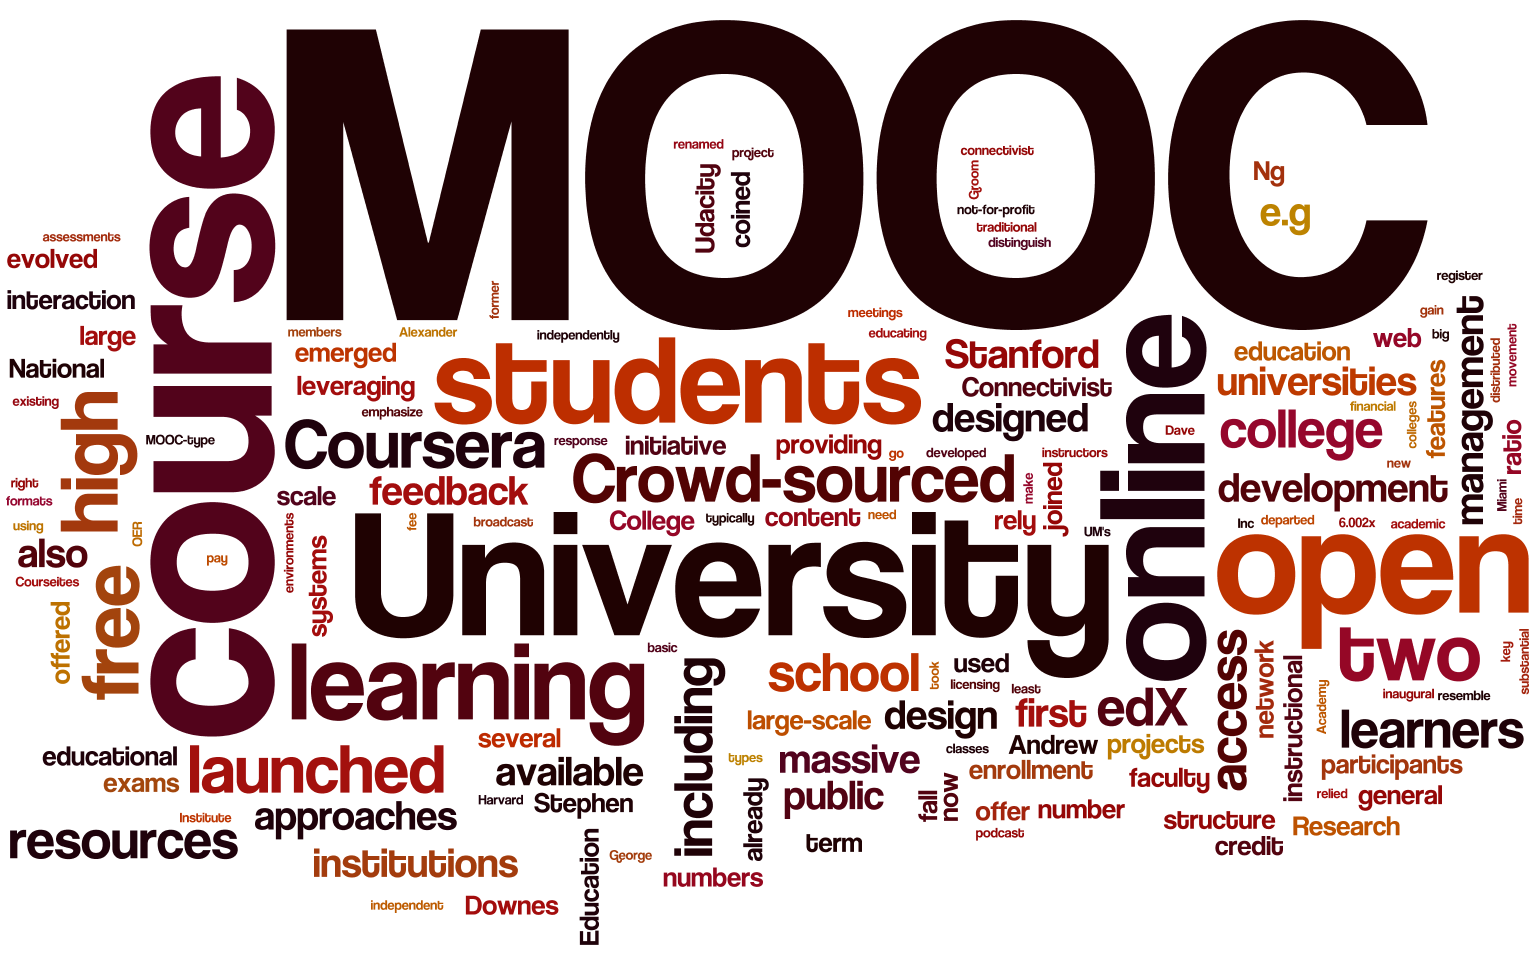
\includegraphics[width=0.7\linewidth]{images/introduction/mooc.png}\hfill
 \caption[Mooc image]{Mooc image}
 \label{fig:fourV}
\end{figure}


Despite the arrival of HTML5, video management is still very insidious. In fact, there isn't a video streaming standard that can ensure the fruition of the contents of the different web browsers and mobile devices.



In fact the lack of protocols shared by the vendor, together with the huge amount of data that must be managed by confronting video content, are a technological obstacle to face and overcome.

The creation of an e-learning service also requires a heavy investment to cover the costs of implementation, storage, and most importantly network traffic required for video content streaming.


The goal of this thesis work at the CVDLAB was to deepen methods and technologies to help overcome the technological obstacle identified in order to offer the opportunity to users and mainly companies to create their own E -learning platform.


For example, one use of the platform can be a big company that wants to create its own Academy section in which they can train the personnel without having to rely on third parties.

Finally, the concept of usability of the components based on the standard HTML5 Web Components was adopted, which greatly facilitated the creation of a final use case: X-Learning.


E-learning is a platform structured into two distinct parts: one part of administration that is addressed to a user who can manage the teacher staff and introduce courses, and another part for users who require the fruition content instead.


The thesis is divided into two parts, each of which consists of three chapters:
The first chapter provides an overview of the main existing MOOC platforms.

The second chapter describes the services used for the realization of the platform and a brief cost analysis.

The third chapter describes the technologies used for the development of the thesis project.

With the start of the second part of the thesis, the project gets more detailed, especially in the fourth chapter there will be an overview of the architecture and organization of the platform.

In the fifth chapter the focus is on core components made in the project and on how they were made.

The sixth and final chapter presents the conclusions and provides possible future developments, focusing on the issues put into production, not directly addressed during the thesis work.